%Config
\documentclass[12pt,twoside]{article}
\usepackage[spanish,es-tabla]{babel}
\usepackage[a4paper]{geometry}

\usepackage{graphicx}               % Para incluir imágenes
\usepackage{amsmath}                % Para el manejo de matemáticas
\usepackage{url}
\usepackage{float}

\usepackage{xcolor}
\usepackage{listings}

% Definir colores
\definecolor{bgcolor}{RGB}{250, 250, 250} % Fondo claro
\definecolor{commentcolor}{RGB}{0, 128, 0} % Comentarios en verde
\definecolor{keywordcolor}{RGB}{0, 0, 128} % Palabras clave en azul oscuro
\definecolor{stringcolor}{RGB}{163, 21, 21} % Cadenas en rojo oscuro

% Configuración de lstlisting para C++
\lstdefinestyle{modernCpp}{
	language=C++,
	backgroundcolor=\color{bgcolor},
	basicstyle=\ttfamily\small,
	keywordstyle=\color{keywordcolor}\bfseries,
	commentstyle=\color{commentcolor}\itshape,
	stringstyle=\color{stringcolor},
	numbers=left,
	numberstyle=\tiny\color{gray},
	stepnumber=1,
	frame=single,
	tabsize=4,
	breaklines=true,
	showstringspaces=false,
	captionpos=b
}

\title{Autómata Celular Elemental y la regla 30}
\author{Erick Jesse Angeles López}


% Definir un comando para palabras clave
\newcommand{\keywords}[1]{%
	\begin{center}
		\textbf{Palabras clave:} #1
	\end{center}
}

\renewcommand{\baselinestretch}{1}
\setcounter{page}{1}
\setlength{\textheight}{21.6cm}
\setlength{\textwidth}{14cm}
\setlength{\oddsidemargin}{1cm}
\setlength{\evensidemargin}{1cm}
\pagestyle{myheadings}
\thispagestyle{empty}
\markboth{\small{Ángeles López Erick Jesse}}{\small{Automata celular elemental y la regla 30}}
\date{}

\begin{document}
	
	\begin{center}
		
		% Contenido izquierdo - Imagen
		\begin{minipage}{0.17\textwidth}
			\centering
			
\includegraphics[width=0.7\textwidth]{img/ipn_logo.jpg} % Ajusta esta línea
		\end{minipage}
		\begin{minipage}{.55\textwidth}
			\centering
			{\Large Instituto Politécnico Nacional}\\
			{\Large Escuela Superior de Cómputo}
		\end{minipage}
		\begin{minipage}{0.17\textwidth}
			\centering
			
\includegraphics[width=0.9\textwidth]{img/escom_logo} % Ajusta esta línea
		\end{minipage}			
	\end{center}
	
	
	\centerline{\bf Ingeniería en Inteligencia Artificial, Algoritmos Bioinspirados}
	
	\centerline{\bf  Sem: 2025-1, 5BM1, Fecha: FECHA}
	
	\centerline{}
	
	%\centerline{}
	
	
	\begin{center}
		\Large{\textsc{Autómata Celular Elemental y la regla 30}} 
	\end{center}
	\centerline{}
	\centerline{\bf {\textit{Presenta}}}
	\centerline{\bf {Angeles López Erick Jesse\footnote{eangelesl1700@alumno.ipn.mx}}}
	\centerline{}
	\centerline{}
	\centerline{\bf {Disponible en:}}
	\centerline{\text{\url{GITHUB}}}
	
	
	
	
	\newtheorem{Theorem}{\quad Theorem}[section]
	
	\newtheorem{Definition}[Theorem]{\quad Definition}
	
	\newtheorem{Corollary}[Theorem]{\quad Corollary}
	
	\newtheorem{Lemma}[Theorem]{\quad Lemma}
	
	\newtheorem{Example}[Theorem]{\quad Example}
	
	\bigskip
	
	\bigskip
	
	\begin{abstract} 
		
	\end{abstract}
	
	\keywords{}
	
	\clearpage
	
	\tableofcontents
	\clearpage
		
	\section{Introducción}
	
	Los autómatas celulares (AC, de ahora en adelante, por su traducción al inglés: ``Cellular Automaton'') fueron concebidos por John Von Neumann en 1948 mientras buscaba diseñar un sistema capaz de auto-replicarse, es decir, un robot con la capacidad de construir otro robot. Las limitaciones físicas lo llevaron a seguir el consejo de Stanislaw Ulam, quien le sugirió diseñar un modelo matemático discreto con esta capacidad de auto-reproducción \cite{b1}.
	
	Los AC se definen como un conjunto de celdas o células que adquieren diferentes valores según la interacción que se produce entre ellas. Matemáticamente, un AC se describe mediante una 4-tupla:
	
	\begin{equation*} CA = \{L, S, N, f\} \end{equation*}
	
	Donde: 
	\begin{itemize} \item $\boldsymbol{L}$: Espacio dimensional. Define la dimensionalidad de una rejilla de células agrupadas. Este espacio es (teóricamente) infinito.

		\item $\boldsymbol{S}$: Conjunto finito de estados que puede adquirir cada célula dentro del espacio asignado.
		
		\item $\boldsymbol{N}$: Define las posiciones relativas de cada célula que formarán parte de la vecindad. El comportamiento de cada célula depende de su vecindad.
		
		\item $\boldsymbol{f : S^{[N]} \rightarrow S}$: Función de transición. Determina el próximo valor de cada célula en función de los valores de las células vecinas. Esta actualización se realiza de manera simultánea en cada periodo de tiempo discreto.
	\end{itemize}
	
	Estos sistemas han sido usados en el modelado de estaciones de metro \cite{b2}, comportamiento de plagas en ecosistemas \cite{b3}, sistemas de mercado financiero \cite{b4} o en el análisis de comportamiento de células cancerígenas \cite{b5}.
	
	Dos de los AC más conocidos son el Juego de la Vida, propuesto por John Conway, y el Autómata Celular Elemental, desarrollado por Stephen Wolfram.
	
	El Juego de la Vida de Conway consiste en un conjunto de células en un espacio bidimensional, un conjunto de estados binarios (vivo y muerto), una vecindad de Moore (las 8 células circundantes) y una función que define la vida o muerte de cada célula con base en la población viva de su vecindad \cite{b6}.
	
	Por otro lado, el Autómata Celular Elemental es una colección de autómatas que comparten un espacio unidimensional, un conjunto de estados binarios y una vecindad de radio uno (la célula en cuestión y sus dos células vecinas más cercanas). Dichos autómatas se diferencian únicamente en la función de transición, que puede adoptar hasta 256 ``reglas'' o configuraciones diferentes \cite{b7}.
	
	Una de estas reglas, conocida y patentada por Wolfram como Regla 30, presenta un comportamiento errático y aparentemente aleatorio. Si se inicia con una única célula viva, esta se expande en ambas direcciones con cada iteración, siendo capaz de llenar todo el espacio. Sin embargo, el comportamiento de la célula inicial no parece seguir un patrón discernible \cite{b8}. Ademas, no parece existir una tendencia de un estado sobre el otro.
	
	Por ello, en este reporte se propone un análisis estadístico sobre el primer millón de generaciones, esto con el objetivo de encontrar un patrón en la frecuencia de aparición de unos y ceros cada cierta segmentación.
	
	\clearpage
	\section{Marco Teórico}
	
	\subsection{Autómata Celular Elemental}
	
	El autómata celular elemental (ECA, de ahora en adelante, por su traducción al inglés: ``Elementary Cellular Automaton'') se caracteriza por su simplificación de los autómatas celulares y su comportamiento divergente.
	
	Sus características principales son:
	\begin{itemize}
		\item Una dimensión: $L = 1$. Es decir, las células están agrupadas en una línea infinita de forma consecutiva.
		
		\item Dos estados posibles por célula: $S = \{0, 1\}$.  
		
		\item Vecindad local: La vecindad de cada célula se define por sí misma y sus dos vecinas más cercanas, también llamado radio 1. La posición relativa está dada por $N = \{-1, 0, 1\}$.  
		
		\item Funciones de transición: Dado que la vecindad está conformada por tres células y cada célula puede adquirir dos valores, existen $|S|^{|N|} = 2^3 = 8$ combinaciones posibles de vecindad. Además, como cada combinación puede tener dos reglas de producción, es decir, generar un 0 o un 1, existen $|S|^{|S|^{|N|}} = 2^{2^3} = 2^8 = 256$ autómatas celulares diferentes.  
		
	\end{itemize}
	
	A cada combinación de vecindad se le puede asociar un número binario determinado por el valor de cada célula. Dado que existen 8 combinaciones, cada ECA se puede representar mediante un número binario de 8 dígitos, lo que, traducido a base decimal, adquiere un valor (y el nombre del ECA) entre 0 y 255.
	
	En la figura \ref{img:eca1}, se muestra la configuración de la regla 210, que equivale a $210_{10} = 11010010_2$ en base binaria. Las casillas negras representan los unos, y las blancas, los ceros.
	
	\begin{figure}[H]
		\centering
		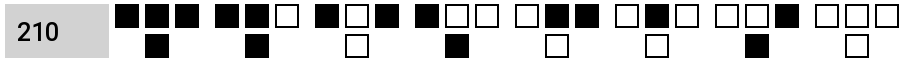
\includegraphics[width=\textwidth]{img/eca1.png}
		\caption{ECA 210}
		\label{img:eca1}
	\end{figure}
	
	El resultado de dicha regla se muestra en la figura \ref{img:eca2}. Se utiliza una segunda dimensión para representar el historial de la regla, aunque el comportamiento afecta únicamente la dimensión original.
	
	\begin{figure}[H]
		\centering
		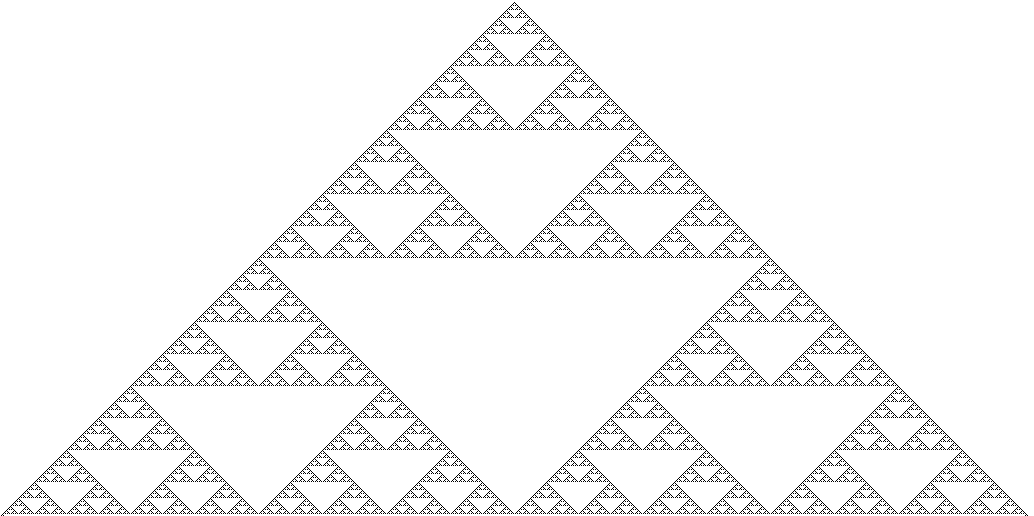
\includegraphics[width=\textwidth]{img/eca2.png}
		\caption{Evolución del ECA 210}
		\label{img:eca2}
	\end{figure}
	
	\subsection{Regla 30}
	
	La regla 30 equivale a $30_{10}=00011110_2$ en binario. Dada una única célula con valor 1, esta se expande en ambas direcciones con cada iteración, como se muestra en las figuras \ref{img:r30_1} y \ref{img:r30_2}, que ilustran las primeras 23 y 900 generaciones, respectivamente.
	
	Como se observa en la figura \ref{img:r30_2}, existe un pequeño patrón repetitivo que crece de forma diagonal en el lado izquierdo del historial. Sin embargo, en el lado derecho, el comportamiento no parece tener estabilidad ni un patrón discernible. Si almacenamos el historial de los valores de la célula inicial, se obtiene una secuencia pseudoaleatoria.
	
	Hasta el momento no se ha podido predecir directamente si el siguiente estado será 0 o 1, es posible calcularlo realizando todas las generaciones previas.
	
	\begin{figure}[H]
		\centering
		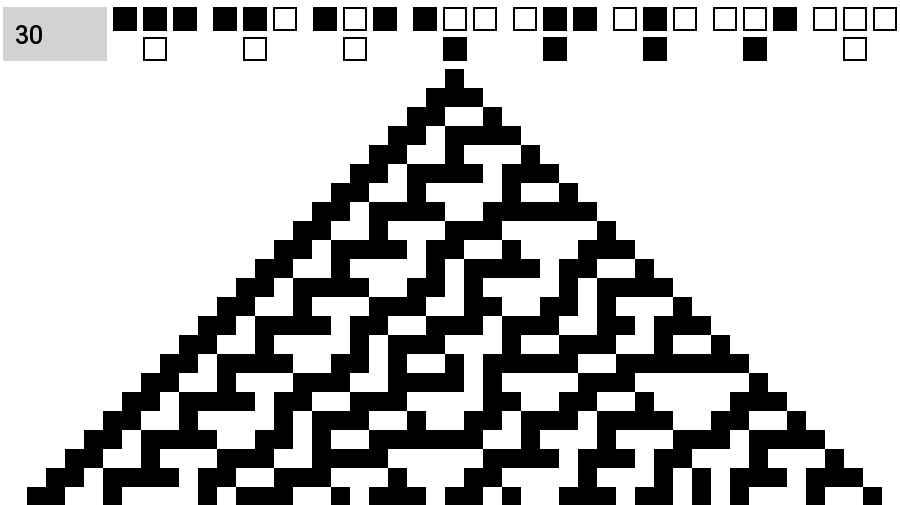
\includegraphics[width=\textwidth]{img/r30_1.png}
		\caption{Primeras 23 generaciones de la regla 30}
		\label{img:r30_1}
	\end{figure}
	
	\begin{figure}[H]
		\centering
		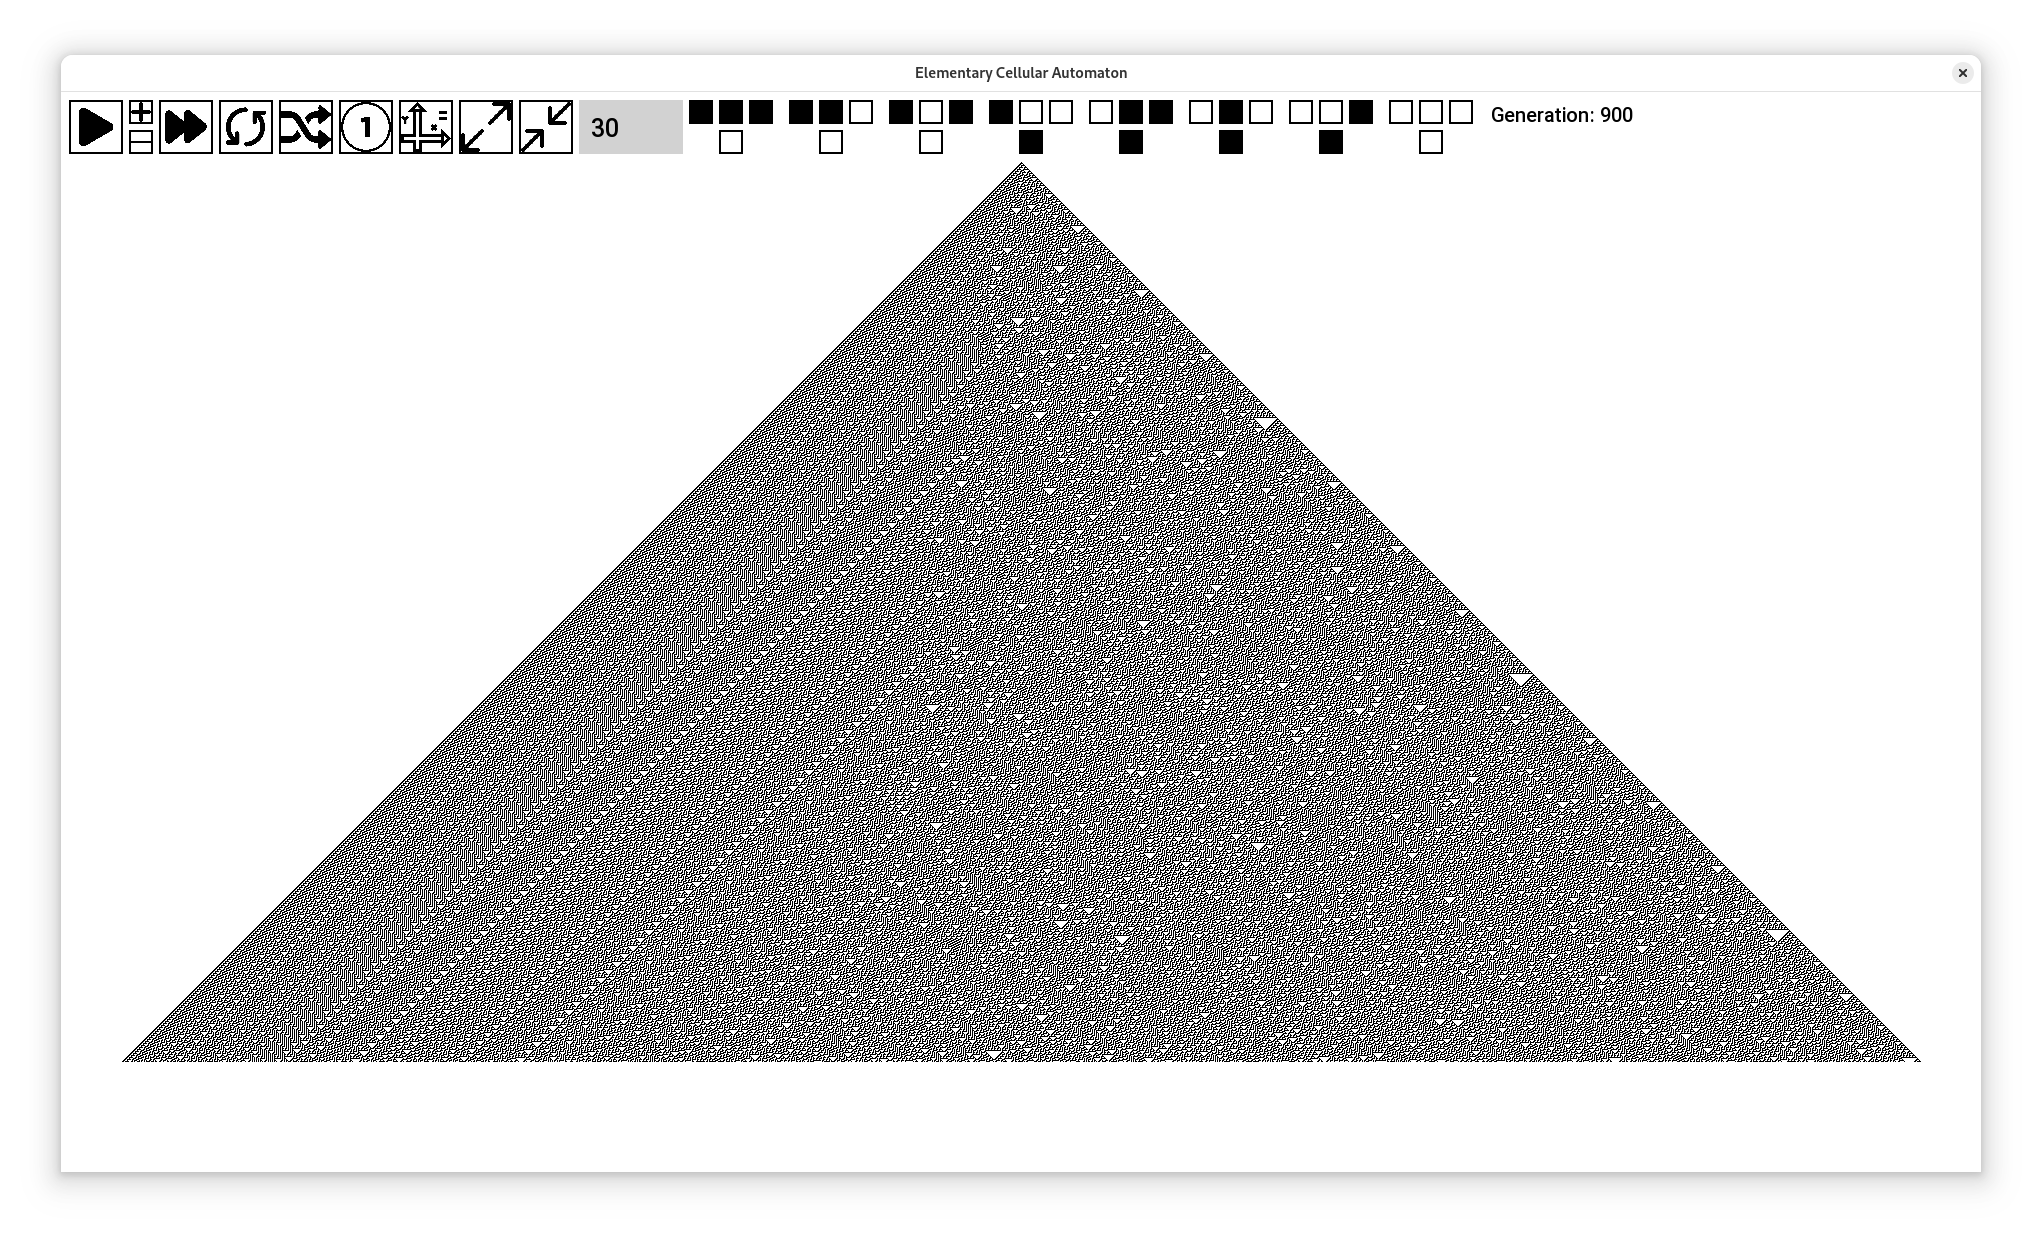
\includegraphics[width=\textwidth]{img/r30_2.png}
		\caption{Primeras 900 generaciones de la regla 30}
		\label{img:r30_2}
	\end{figure}
	
	\section{Metodología}
	
	\subsection{Producción de generaciones}
	
	Debido al computo intensivo requerido, se diseño un programa en C++ que permite generar, cifrar y almacenar cada nueva generación en un archivo binario. Cada generación se componen de una secuencia de valores booleanos (equivalente a binario), por lo que se agrupan en octetos para formar bytes.
	
	Las generaciones se almacenan en archivos diferentes para poder acceder a ellas de forma independiente. Esto permite que, dada una generación $n$, se pueda calcular la generación $n + 1$ sin la necesidad de almacenar las $n - 1$ generaciones anteriores. 
	
	El número de operaciones depende del tamaño del vector, y dado que cada nueva generación aumenta en dos unidades y tiene una longitud impar, se puede utilizar la fórmula de la suma de Gauss para números impares:
	
	\begin{equation*}
		\sum_{i = 1}^{n} 2i - 1 = n^2
	\end{equation*}
	
	Fueron requeridos 6.25 millones de operaciones para producir 2.5 millones de generaciones almacenadas en 782 GB.
	
	Sea la actual generación de tamaño $m$, se crea un vector de tamaño $m + 2$ y se itera sobre cada elemento para obtener el nuevo valor aplicando la regla 30 a la vecindad como se muestra en el fragmento de código \ref{step}. Finalmente se codifica y se almacena en un archivo de tipo binario.
	
	Finalmente, se extra el valor de la columna principal de cada generación para formar el vector de interés.
	
	\begin{lstlisting}[style=modernCpp, caption=Ejemplo de código en C++,  label=step]
		#include <iostream>
		
		int main() {
			std::cout << "Hola, mundo!" << std::endl; // Imprime un mensaje
			return 0;
		}
	\end{lstlisting}
	
	\subsection{Extracción de características}
	
	

	Se diseñó una función que itera sobre todas las generaciones actualmente cargadas y extrae el valor de la columna principal, es decir, el valor en la posición $n$. Este procedimiento se realiza para todas las generaciones, hasta obtener un vector de valores booleanos que, a su vez, se reescribe en un archivo binario.
	
	Además, se generan previamente los primeros $m$ números primos menores a 1,250,000 para evitar calcularlos en tiempo de ejecución. Se define este tamaño ya que es el numero máximo que un vector de 2.5 millones puede ser dividido en mas de una unidad entera.
	
	\subsection{Múltiplos primos}
	
	El vector de datos de la columna principal se divide en sub-vectores, cada uno del mismo tamaño $n$. Posteriormente, se almacena la frecuencia del estado 1 en cada sub- con el objetivo de extraer la frecuencia de esta estado en cada partición del vector original. Este paso se repite generando sub-vectores de todos los tamaños $n$ menores a 1.25 millones, ya que es el segundo divisor mas grande de 2.5 millones.
	
	Por el teorema fundamental de la aritmética, todo número puede expresarse como el producto de números primos. Por esta razón, no es necesario calcular las frecuencias de todos los $n$ menores a 1.25 millones, sino unicamente de todos aquellos números primos menores a 1.25 millones. Si existe un patrón en la frecuencias, dicho patrón se espera estar presente  en las frecuencias de sus componentes primarias.
	
	\subsection{Histograma}
	
	
	
	\clearpage
	\addcontentsline{toc}{section}{Referencias}
	\begin{thebibliography}{99}
		\bibitem{b1}
		M. G. Magaña Chávez. ``Autómatas celulares elementales y sus composiciones''. Motivos matemáticos / Matemáticas aplicadas. Accedido el 24 de diciembre de 2024. [En línea]. Disponible: \url{https://motivos.matem.unam.mx/vol6/num1/aplicadas1.html#:~:text=En%201948,%20el%20célebre%20matemático,de%20construir%20a%20otro%20robot}
		
		\bibitem{b2}
		C. A. Rodríguez Garzón, ``Modelamiento de estaciones TransMilenio mediante Autómatas Celulares: lecciones aprendidas'', Ingeniería, vol. 19, n.º 2, diciembre de 2014. Accedido el 28 de diciembre de 2024. [En línea]. Disponible: \url{https://doi.org/10.14483/udistrital.jour.reving.2014.2.a05}
		
		\bibitem{b3}
		V. E. Barros Arenas y H. Gilabert P., ``Modelación de la dinámica Plaga-Parasitoide-Bosque mediante autómatas celulares'', Cienc. \& Investig. For., vol. 14, n.º 2, pp. 311–323, julio de 2008. Accedido el 28 de diciembre de 2024. [En línea]. Disponible: \url{https://doi.org/10.52904/0718-4646.2008.292}
		
		\bibitem{b4}
		J. J. M. Martínez, ``Modelo de autómatas celulares para la dinámica de un mercado financiero'', Económica, pp. 46–94, diciembre de 2018. Accedido el 28 de diciembre de 2024. [En línea]. Disponible: \url{https://doi.org/10.24215/18521649e004}
		
		\bibitem{b5}
		T. Muñoz Jiménez, A. Torres Soto y M. D. Torres Soto, ``Autómatas Celulares Aplicados al Comportamiento de Células de Cáncer Cervicouterino'', Tecnol. Educ. Rev. CONAIC, vol. 6, n.º 1, pp. 44–49, enero de 2021. Accedido el 28 de diciembre de 2024. [En línea]. Disponible: \url{https://doi.org/10.32671/terc.v6i1.48}
		
		\bibitem{b6}
		``Conway's Game of Life - LifeWiki''. Conway's Game of Life. Accedido el 25 de diciembre de 2024. [En línea]. Disponible: \url{https://conwaylife.com/wiki/Conway's_Game_of_Life}
		
		\bibitem{b7}
		Wolfram Research, Inc. ``Elementary Cellular Automaton''. Wolfram MathWorld. Accedido el 28 de diciembre de 2024. [En línea]. Disponible: \url{https://mathworld.wolfram.com/ElementaryCellularAutomaton.html}
		
		\bibitem{b8}
		Wolfram Research, Inc. ``Rule 30''. Wolfram MathWorld. Accedido el 28 de diciembre de 2024. [En línea]. Disponible: \url{https://mathworld.wolfram.com/Rule30.html}
		
	\end{thebibliography}
	
\end{document}
